\documentclass[a4paper,12pt]{jarticle}
\usepackage[top=20truemm,bottom=20truemm,left=20truemm,right=20truemm]{geometry}
\usepackage[dvipdfmx]{graphicx}
%\usepackage{here}
\usepackage[utf8]{inputenc}
\title{情報と産業・社会 レポート1 課題1}
\author{学生番号\\氏名}
\date{平成29年7月25日}
\begin{document}
\maketitle
\tableofcontents
\section{はじめに(目的)}
%文章で4~5行程度にまとめる。
%「課題」についての背景、経緯、目的などを述べる。
%「まとめ(結論)」と対応させる。
課題:\\
携帯電話やスマートフォンのみ使う群と、ネットにつながったコンピュータを使う群とで、情報リテラシーに差がつくとしたらどのような点か、考察せよ。\\
%情報リテラシーの定義も記述する。
\\
以下のことについて調べることを目的とする。
%\begin{itemize}
%\item 現在どのような情報セキュリティに絡んだ犯罪の形態があるのかを知る。
%\item そのような形態の犯罪に対してどのような対策が考えられるのかを知る。
%\item より一般的にあらゆる情報セキュリティに絡んだ犯罪に対してどのような対策が考えられるのかを知る。
%\end{itemize}
\section{調査方法}
%具体的な調査方法を箇条書き、または図(絵)を使ってわかりやすく説明する。
%2ページ以内でまとめる。
インターネットを使用して調査した。
\begin{center}

\includegraphics[width=100truemm]{computer_search_kensaku.png}
\end{center}
\section{調査結果}
%調査結果を箇条書き、または図(グラフ)を使ってわかりやすく説明する。
%2~3ページ程度にまとめる。
%\begin{description}
% \item[調査対象]\mbox\\\\
% 今回は最近世界各国で攻撃を行っている暗号化型ランサムウェアWannaCryについて調査した。
% \item[ランサムウェアとは?]\mbox\\\\
% マルウェアの一種で、感染したPCをロックしたり、ファイルを暗号化したりすることによって使用不能にしたのち、元に戻すことと引き換えに「身代金」を要求する。身代金要求型不正プログラムとも呼ばれる。スパムメールや改竄した正規サイトから脆弱性を攻撃する不正サイトへ誘導され、感染する。ランサムウェアに感染すると、特定の機能を無効化して操作不能にしたり、ファイルを暗号化して利用不能にする。そして感染前の状態に復元することと引き換えに金銭の支払いを要求する画面が表示される。
%  \begin{figure}[H]
%   \begin{center}
%    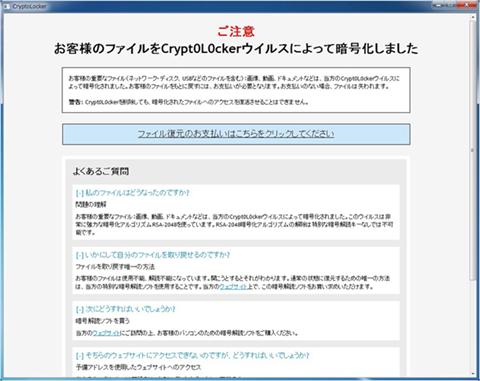
\includegraphics[width=100truemm]{Ransomware.png}
%    \caption{ランサムウェアに感染した時に表示される支払い要求画面の例}
%    \label{RansomwarePicture}
%   \end{center}
%  \end{figure}
% \item[暗号化型ランサムウェアWannaCry]\mbox\\\\
% ランサムウェアによる被害は2015年から2016年にかけて爆発的に増えたが、先月からその被害が世界各地で報告されている「WannaCry」は、たったひとつのランサムウェアが短期間に多くの被害者を出したことで注目されるようになった。
%  \begin{figure}[H]
%   \begin{center}
%    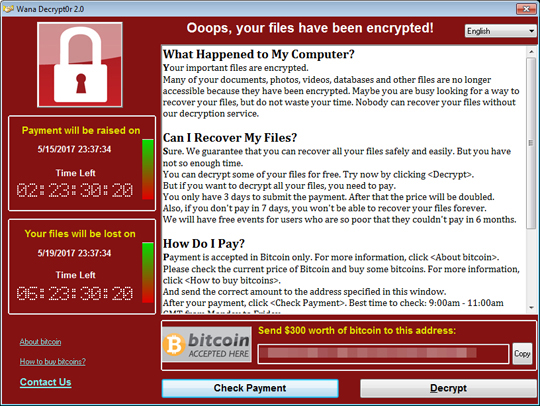
\includegraphics[width=100truemm]{WannaCry.jpg}
%    \caption{WannaCryの脅迫画面}
%    \label{WannaCryPicture}
%   \end{center}
%  \end{figure}
% WannaCryが侵入すると、不正ファイルを実行して自分自身を感染拡大させ、暗号化を行う不正ファイルと脅迫状を表示するファイルを作成し、ローカルフォルダ及び共有フォルダ内のファイルを暗号化して脅迫状を表示し、一週間以内の300ドル分のビットコインの支払いを要求する。
%  \begin{figure}[H]
%   \begin{center}
%    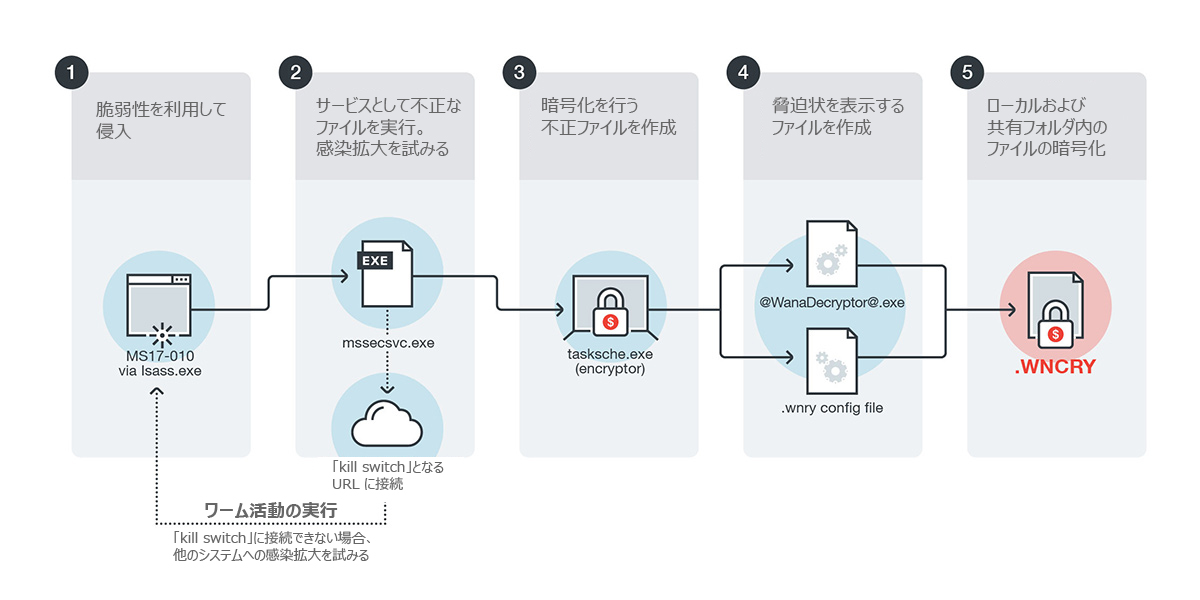
\includegraphics[width=150truemm]{WannaCryFlow.jpg}
%    \caption{WannaCryによる暗号化・脅迫の流れ}
%    \label{WannaCryFlowPicture}
%   \end{center}
%  \end{figure}
% \item[WannaCryなどのマルウェアに対する効果的なセキュリティ対策]\mbox\\\\
% 今回調査したWannaCryはWindowsの古いバージョンへの感染しか確認されておらず、OSのアップデートを行うことで十分な対策となる。既存のソフトウェアの中に日々新たな脆弱性が見つかり、その脆弱性を狙うマルウェアが日々発生しているので、OSやセキュリティ対策ソフトウェアを常に最新版にしておくことが有効である。
%\end{description}
\section{考察}
%自分がどう考えたか(意見)を根拠(理由)とともに述べる。
%箇条書きで記載する。
%\begin{itemize}
% \item ITの発達と犯罪について
% ITが発達じた現代においては、大量の情報を瞬時に処理できたり、情報を用意に世界中に発信することができるようになり、人間ができることの可能性が広がり、これからも更に広がり続けると予想されるが、それは同時に犯罪の可能性も広がっていく、多様化していくということになる。WannaCryのようなたったひとつのコンピュータウイルスが世界中に影響を与えることになったのもITが発達した結果である。IT産業に従事する人たちも、ITを利用する人たちも、このことに注意してITに関わるべきだと考える。
%\end{itemize}
%\newpage
\section{まとめ(結論)}
%文章で箇条書きに記載する。
%「はじめに(目的)」と対応させる。
%\begin{description}
% \item[現在どのような情報セキュリティに絡んだ犯罪の形態があるのかを知る。]\mbox\\\\
% WannaCryを例として調査し、ランサムウェアという形態を知った。
% \item[そのような形態の犯罪に対してどのような対策が考えられるのかを知る。]\mbox\\\\
% OSやセキュリティ対策ソフトウェアを常に最新版にしておくという対策、およびそれがなぜ有効であるかを知った。
% \item[より一般的にあらゆる情報セキュリティに絡んだ犯罪に対してどのような対策が考えられるのかを知る。]\mbox\\\\
% ITの発達は同時に犯罪の発達でもあるということに注意してITと関わるという対策を知った。
%\end{description}
\section{参考文献}
%題目、著者名、雑誌(書籍)名、年号、ページを必ず記載する。
%\begin{thebibliography}{99}
% \bibitem{WannaCry1} 大規模な暗号化型ランサムウェア「WannaCry/Wcry」の攻撃、世界各国で影響 http://blog.trendmicro.co.jp/archives/14873
% \bibitem{WannaCry2} Wanna Cryに攻撃手法を提供した「Shadow Brokers」とは何者か? https://the01.jp/p0005012/
% \bibitem{Ransomware} ランサムウェア http://www.trendmicro.co.jp/jp/security-intelligence/threat-solution/ransomware/
%\end{thebibliography}
\end{document}
